
{\em La figure ci-contre n'est qu'un     dessin à main levée.}

\begin{wrapfigure}[7]{r}{7cm}
\vspace{-7mm}
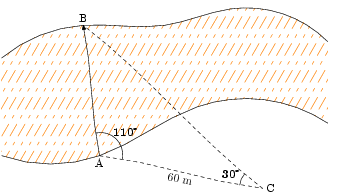
\includegraphics[scale=1]{TR-exo32.png} 
\end{wrapfigure}   

    
    On souhaiterait connaître la largeur de la
  rivière, c'est-à-dire la longueur $AB$, mais on ne dispose d'aucun
  moyen pour traverser.

  \begin{enumerate}
    \item A l'aide d'un décamètre et d'un goniomètre, on a obtenu des
      indications portées sur la figure ci-contre. Construis un dessin
      à l'échelle 1/1\,000 de cette situation. Pour cela :
      \begin{itemize}
      \item Construire le segment $[AC]$;
      \item Construire les angles $\widehat{ACB}$ et $\widehat{CAB}$
        avec un rapporteur;
       on obtient alors le point $B$ (vérifie la mesure de
        l'angle $\widehat{ABC}$);
      \item Déterminer alors la longueur $AB$ {\em réelle}, sur le terrain.
      \end{itemize}
  \end{enumerate}

\begin{enumerate}
    \item Pour obtenir une valeur plus précise :
      \begin{itemize}
      \item Reconstruire le triangle $ABC$ et trace la hauteur issue de
        $A$. Elle coupe le segment $[BC]$ en $H$.
      \item Déterminer la mesure de l'angle $\widehat{CAH}$ puis
        calcule la longueur $AH$.
      \item Déterminer la mesure de l'angle $\widehat{ABC}$ puis la
        mesure de l'angle $\widehat{BAH}$.
      \item Calculer alors la longueur $AB$.
      \end{itemize}
  \end{enumerate}
 